% Refer to https://web.evanchen.cc/faq-latex.html
\documentclass[11pt]{article}
\usepackage{tabularray, xcolor, xurl, minted, evan}
\usepackage[backend=biber]{biblatex}
\addbibresource{Ref.bib}
\usepackage{tocloft}  % For customizing Table of Contents

% Colours
\definecolor{lightgray}{gray}{0.963}

% 1. Adjust the gap between subitems in the Table of Contents
\setlength{\cftsubsecskip}{0.5ex}  % Adjust spacing between subsections
\setlength{\cftsubsubsecskip}{0.3ex}  % Adjust spacing between subsubsections (if needed)

% 2. Apply \sffamily font to top-level sections in the Table of Contents
\usepackage{hyperref}  % Optional for clickable links
\usepackage{titlesec}   % For section title customization

\titleformat{\section}{\sffamily\Large\bfseries}{\thesection}{1em}{}

% Customizing the Table of Contents
\renewcommand{\contentsname}{\sffamily\bfseries Contents}
\renewcommand{\cftsecfont}{\sffamily\bfseries}  % Apply \sffamily to sections in TOC
\renewcommand{\cftsecpagefont}{\sffamily\bfseries}  % Apply \sffamily to section page numbers in TOC

\fancyhead[L]{\sffamily M3 Maths Challenge 2025}  % Custom text on the left of the header
\fancyhead[C]{\thepage} % Current page no
\fancyhead[R]{\sffamily Team \#17559}  % Custom text in the center of the header

\hypersetup{
  colorlinks = true,
  urlcolor   = blue,
  linkcolor  = blue,
}

% Make all headings sans-serif
\usepackage{titlesec}
\titleformat{\section}{\sffamily\Large\bfseries}{\thesection}{1em}{}
\titleformat{\subsection}{\sffamily\large\bfseries}{\thesubsection}{1em}{}
\titleformat{\subsubsection}{\sffamily\normalsize\bfseries}{\thesubsubsection}{1em}{}
\titleformat{\paragraph}{\sffamily\normalsize\bfseries}{\theparagraph}{1em}{}

% Make title sans-serif
\makeatletter
\renewcommand{\maketitle}{
    \begin{center}
        {\sffamily\bfseries\LARGE \@title} \\[1em]
        {\sffamily\large \@author} \\[1em]
        {\sffamily\large \thedate} \\[1em]
    \end{center}
    \vspace{1em}
}
\makeatother

\title{M3 Maths Challenge: \textit{Staying Cool as the World Heats Up}}
\author{Team \#17559}

\begin{document}
\maketitle

\section{Executive Summary}

Indeed it is no secret that global warming is going to have massive implications on global temperatures, a cities' economy and
the overall health of a city's population. In this paper we explore these 3 domains and analyse the extent of the effect that
global warming has using various mathematical models implemented in the Python programming language.

Our team investigates how global warming is affecting Birmingham, England, currently and years to come using the predictions
from our models and by analysing past data.
\vspace{0.3cm}

In Q1 we were asked to predict the indoor temperatures for resedential homes in without air conditioning over a time period of
24 hours during a heatwave. We use the dataset given \cite{m3} to create a multivariate polynomial regression model of degree
3 in order to predict indoor temperatures $t$ seconds after midnight. We have developed a Python program that implements a
function called \texttt{Predict\_Temps(new\_data, year)} that predicts temperatures over the course of 24 hours and produces a
list of predicted temperatures across each hour in the entire 24 hours. A complete concrete list of predicted temperatures
per hour can be viewed at the end of section \ref{sec:results1}.

In Q2 we were asked to predict the peak demand of energy consumption in kWh now and 20 years from now. We implement the
Holt-Winters exponential smoothing model in Python in order to make predictions for these values. From our predictions we
conclude that the peak energy demand that Birmingham should be prepared to handle now is $2.76 \times 10^8$ kWh, and in 20
years from now the value will be $2.68 \times 10^8$ kWh.

Finally in Q3 we were asked to find a suitable 'vulnerability scale' that could be assigned to any sub-city within Birmingham which would then allow city officials to determine the amount of resources allocated to these particular areas in the event of a heat wave or power grid failure. We decided to calculate the heat index values via Python in order to model how these values would look for the actual heat wave for the data that M3 provides. From this data, we can suggest to city officials that some of the power of the UK, given that they are affected to a lesser extent by the heat waves, should be directed to irmingham during the heat wave in order to allow most of the population, i.e. the ones who have access to AC, to activate it to minimize the effects of any heat stroke and also by providing this excess power it prevents any power outages or power grid failures.

\newpage
\tableofcontents
\newpage

\section{Q1: Hot to Go}

\subsection{Problem Statement}

In Q1 we interpret the problem statement like so:

Predict indoor temperatures for resedential homes without air conditioning over a time period of
24 hours, in Birmingham England, during a heatwave.

\subsection{Assumptions}

\textbf{\sffamily We assume that all homes are made from bricks or another similar material.}

\textit{Justification:} For this question we have selected to analyse homes in Birmingham, England. It is intuitive
to reason that all homes are built out of bricks, concrete or some other similar material. Indeed we understand that
the United Kingdom is considered to be an advanced developed country, with the 6th largest economy by nomial GDP, as
of October 2024 \cite{imf}, so it is reasonable to assume that most of these homes are built from bricks.

\noindent
\textbf{\sffamily We assume that the heatwave is the only natural disaster occuring throughout the entire 24 hours.}

\textit{Justification:} If another natural or manmade disaster happens to occur during that 24 hour time frame the temperatures
could fluctuate greatly without pattern, indeed if a heatwave occurs at the same time as another natural disaster it
would introduce too large of an uncertainty in the accuracy of our model, Hence we simplify our task by assuming
that the only disaster is the heatwave.

\noindent
\textbf{\sffamily We assume that the rate of global warming is constant.}

\textit{Justification:} Since the rate of global warming is dependent on numerous factors that are outside of our control we
choose to assume that the rate of global warming is a constant value.

\subsection{Analysing the problem}

Indeed the temperature inside a given home will vary based on a number of environmental and non-environmental
factors. It is well known that temperatures throughout the day naturally peak around midday and tend to fall off in
the early morning and late at night. This motivates an intuition for a model with a shape similar to the bell curve
shape of a normal distribution.

\[
f(x) = \frac{1}{\sigma \sqrt{2\pi}} \exp \left( -\frac{1}{2} \left( \frac{x-\mu}{\sigma} \right)^2 \right)
\]

\noindent
However the behaviour of such a curve is not so easy to modify when we are given a good number of variables, like in
this problem. We instead make use of \textit{multivariate polynomial regression} to find a polynomial that can
accurately model the variation of temperatures in a room given $n$ parameters, using a Python program.

\subsection{Variables and parameters}

\begin{longtblr}[
  caption={Variables and parameters.}
]{
  colspec={llX},
  row{1}={lightgray}
}

Name & Notation & Description \\

Outside temperature & $T$ & Average outside temperature measured in degrees celcius. \\

Dew point & $D$ & The outside dew point measured in degrees celcius. \\

Humidity & $\zeta$ & Relative humidity expressed as a percentage, where 100\% means the air is fully saturated with moisture, and values at 0\% indicate the air is not saturated. We let 100\% be 1 and 0\% be 0 such that $\zeta \in [0,1]$. \\

Time & $t$ & The time in seconds after 00:00 (midnight).\\

Year & $Y$ & The current year. \\

\end{tblr}

\subsection{Developing the model}

Define $\theta(T, D, \zeta, t)$ to be the function that predicts an indoor temperature
during a heatwave in Birmingham, England. Since we have 4 variables it is easy to see that our function will have
$\binom{n+4-1}{4-1}$ terms as a consequence of stars and bars. So $\theta$ is a multivarite polynomial of degree $n$ the
following form,

\[
  \sum_{ \substack{e_T + e_D + ... + e_t = n \\ 1 \leq r \leq \binom{n + 4}{4}}} \lambda_r T^{e_T} D^{e_D} \cdots t^{e_t}
\]

Indeed global warming is causing the average temperature to increase each year. According to the
\textit{National Oceanic and Atmospheric Administration} (NOAA) earth's average temperature has been increasing by 0.06
degrees celcius each decade since 1850 \cite{noaa}. So we make use of our assumption that the rate of global warming is constant and
redefine $\theta$ to be that summation plus $(Y-2025)0.006$.

A first degree polynomial would be to simple and hence unsuitable to model the curves and other features that we
might find in a graph of temperature against time. A second degree polynomial may be able to capture basic
trends in the data. Using a polynomial of a very high degree will cause the $\binom{n+3}{3}$ term to grow extremely
quickly, meaning that an algorithm would to find our coefficients $\lambda_i$ would run very slowly. Furthermore usage of a
high polynomial degree could potentially lead to our model \textit{overfitting} to our dataset, potentially reducing the
final accuracy of our model. So instead we simply use a degree 3 polynomial. We fit our model against the data given in the data set provided by M3.
\cite{m3}

We use linear regression to find our coeffecients with the Python Scikit-learn library, and then plot the residuals against
the data set that we trained against to evaluate the performance of our model. Here is a snippet of the code.
\textit{See the appendix for the entirety of the code.}

\begin{minted}[bgcolor=lightgray, linenos, breaklines]{python}
# Degree of our polynomial
DEG = 3

# Data given by M3
data = {
    ...
}

df = pd.DataFrame(data)

...

# Create a pipeline that first transforms the features into polynomial features
# then fits a linear regression model
model = make_pipeline(PolynomialFeatures(degree=DEG, include_bias=False), LinearRegression())

# Fit the model
model.fit(X, y)

# To see the learned coefficients, we can extract them from the LinearRegression step
lin_reg = model.named_steps['linearregression']
print("Intercept:", lin_reg.intercept_)
print("Coefficients:", lin_reg.coef_)

# Predict on the entire dataset to test it
y_pred_all = model.predict(X)
residuals = y - y_pred_all

...
plt.show()
\end{minted}

Here are the outputs, the predicted temperatures start from 00:00 and increase by 1 hour each time. So the first value gives
temperature in degrees celcius at 00:00 then the second gives temperature at 01:00 and so on.
\label{sec:results1}
\begin{minted}[bgcolor=lightgray]{text}
Intercept: -1275787.4333442824
Coefficients: [-6.23973942e-23 -1.96969079e-19 -6.91442636e-19  2.46451279e-13
  4.92628196e-17  3.53635378e-18 -6.75490063e-21 -3.27335745e-22
  9.75228429e-26  4.16915770e-23  1.93397873e-19 -2.40666684e-18
  2.66786448e-11  1.29282060e-12 -3.88232972e-16 -2.64492896e-19
 -1.08428510e-20 -2.27176515e-22  5.27294229e-24]

Predicted Temperatures: [21.76129363 18.76824161 17.05217446 17.06800382 16.46977547 16.48559558
  17.18668672 27.66137863 29.69367947 33.46963231 34.61344218 35.62198628
  35.65301066 35.78871563 35.5220175  34.25571878 34.2714295  33.68865326
  32.57605841 32.59175584 27.90601002 27.9216973  27.93737816 26.53566475]
\end{minted}

\begin{center}
\begin{figure}[H]
  \centering
  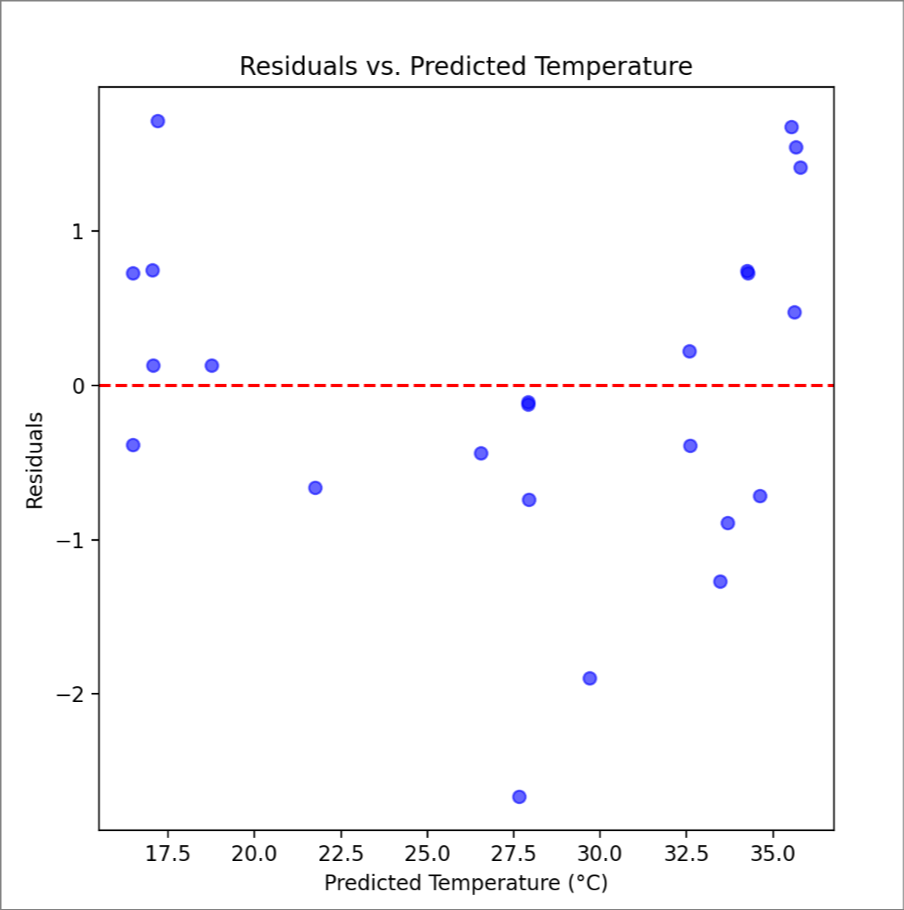
\includegraphics[scale=0.3]{Images/Q1.png}
  \caption{Plot of the residuals against the data set given.}
\end{figure}
\end{center}

\subsection{Discussion of results}

By analysing our Matplotlib graph, we find that we have a discrepency of at most 1-2 degrees celcius when predicting
temperatures. This demonstrates that our model produces relatively accurate values with minimal error. The strengths of this
model include the fact that it can potentially be improved significantly by simply changing the degree that we use in our
approximation, and that we are able to produce a clear visualisation to present the accuracy of our predicitons each time.
Since our output coefficients ended up being rather small (most of them were of the order $10^{-11}$ or smaller) this could
introduce a measure of numerical instability in our model. Since computers work with a limited amount of precision it would
certainly be preferable to have coefficients that require less precision in order to be represented.

\section{Q2: Power hungry}

\subsection{Problem statement}

For Q2 we interpret the problem statement like so:

Predict the peak demand of power in kWh that the city’s power grid should be prepared to handle during the summer months,
now and in 20 years from now.

\subsection{Assumptions}

\textbf{\sffamily We assume that no disaster occurs in the time period that we are predicting.}

\textit{Justification:} Disasters both manmade and natural will cause massive fluctuations in the amount of power used, whilst
we have no information to predict when future disasters will occur. For this reason it makes sense to make such an assumption.

\noindent
\textbf{\sffamily We assume that the proportion of electricity consumed in summer months per an entire year is a constant.}

\textit{Justification:} Since we only have data for each year but we instead would like data for the summer months. Since we
don't have data for other months we have to assume that the proportion of energy consumption per year used in the summer
months is a constant value, $\chi$.

\subsection{Analysing the problem}

By studying the dataset given by M3 \cite{m3}, we find that the domestic consumption of electricity seems to be decreasing at
a constant rate with minor fluctuations in between. The non-domestic consumption of electricity seems to have remained
relatively constant from 2012 to 2022 this time with larger fluctuations from 2015 to 2019.

Both of these data sets demonstrate an amount of fluctuation in their overall trends. This motivates an attempt at using a
model that places more emphasis on recent data rather than using a model given by an explicit well defined mathematical
function that would place more emphasis on the long term trends.

In order to achive this we make use of the \textit{Holt-Winters Exponential} smoothing model with an additive time series. This model
takes into account both long term progression (trends) and short term patterns and cycles (seasonality) as well as the
baseline value of our model (level). The model would be of the following form, for $\delta$ time steps in the future the
energy used will be given by

\[ E_{t+\delta} = l_t + \delta b_t + s_{t-T+\delta} \]

where $l_t$ is the level at time $t$, $b_t$ is the trend at time $t$, $s_t$ is the season at time $t$, $E_t$ is the energy
consumption at time $t$ and $T$ is the seasonal period.

We create 2 models one to model the variation in the domestic energy consumption, and one to model the variations in the
non-domestic energy consumption, then sum up these models in order to give a value for resultant energy consumption.

\subsection{Variables and parameters}

\begin{longtblr}[
  caption={Variables and parameters.}
]{
  colspec={llX},
  row{1}={lightgray}
}

Name & Notation & Description \\

Constant of proportionality & $\chi$ & The constant of proportionality of the consumed energy in summer per the total energy consumed per year. \\

Level, Domestic energy & $l_{d, t}$ & The level of the domestic energy at a time $t$. \\

Level, Industrial energy & $l_{i, t}$ & The level of the industrial energy at a time $t$. \\

Trend, Domestic energy & $b_{d, t}$ & The trend of the domestic energy at a time $t$. \\

Trend, Industrial energy & $b_{i, t}$ & The trend of the industrial energy at a time $t$. \\

Season, Domestic energy & $s_{d, t}$ & The season of the domestic energy at a time $t$. \\

Season, Industrial energy & $s_{i, t}$ & The season of the industrial energy at a time $t$. \\

Year & $Y$ & The year of when we want to predict electricity consumed\\
\end{longtblr}

\subsection{Developing the model}

Let $E_d(t)$ be a function of domestic energy consumption for the year $t$ in kWh. Let $E_i(t)$ be a function of industrial
(non-domestic) energy consumption for the year $t$ in kWh. We define $\Sigma (t)$ to be the function that gives the total
energy used at a time $t$, such that $\Sigma(t) = \chi(E_d(t) + E_i(t))$. We make use of the data set given by the M3
\cite{m3}, which only gives energy consumption per year in Birmingham, England except for 2019 where energy consumption is
broken down by month.

By computing the proportion of energy consumed in the summer months of 2019 against the total energy used in 2019 we determine
a value for $\chi \approx 0.081$ that is 8.1\%.

We use the statsmodels library in Python to implement this algorithm, here is a snippet of the algorithm:
\textit{Full code can be viewed in the appendix.}

\begin{minted}[linenos, bgcolor=lightgray, breaklines]{python}
...
# Constant of propotionality (refer to paper)
CHI = 0.081
data["Domestic Consumption"]     *= CHI
data["Non-Domestic Consumption"] *= CHI

...
# Fit Holt-Winters models for each consumption type
domestic_model = ExponentialSmoothing(
    data["Domestic Consumption"],
    trend='add',      # Additive trend since the data is annual
    seasonal=None,    # No seasonal component for annual data
    initialization_method="estimated"
).fit()

nondomestic_model = ExponentialSmoothing(
    data["Non-Domestic Consumption"],
    trend='add',
    seasonal=None,
    initialization_method="estimated"
).fit()

# Compute the fitted values for each model and sum them to get the combined (total) fitted values
data["Total Fitted"] = domestic_model.fittedvalues + nondomestic_model.fittedvalues

# Also, calculate the actual total consumption for comparison
data["Total Actual"] = data["Domestic Consumption"] + data["Non-Domestic Consumption"]

# Forecast the next 20 years using both models and sum their forecasts
forecast_steps = 20
domestic_forecast = domestic_model.forecast(steps=forecast_steps)
nondomestic_forecast = nondomestic_model.forecast(steps=forecast_steps)
total_forecast = domestic_forecast + nondomestic_forecast

...

plt.show()
\end{minted}

Here is the output from the code:

\begin{minted}[breaklines, bgcolor=lightgray]{text}
Forecast for Total Consumption for the next 20 years:
1    2.765753e+08
2    2.761579e+08
3    2.757406e+08
4    2.753233e+08
5    2.749060e+08
6    2.744886e+08
7    2.740713e+08
8    2.736540e+08
9    2.732366e+08
10    2.728193e+08
11    2.724020e+08
12    2.719846e+08
13    2.715673e+08
14    2.711500e+08
15    2.707327e+08
16    2.703153e+08
17    2.698980e+08
18    2.694807e+08
19    2.690633e+08
20    2.686460e+08
\end{minted}

\begin{center}
\begin{figure}[H]
  \centering
  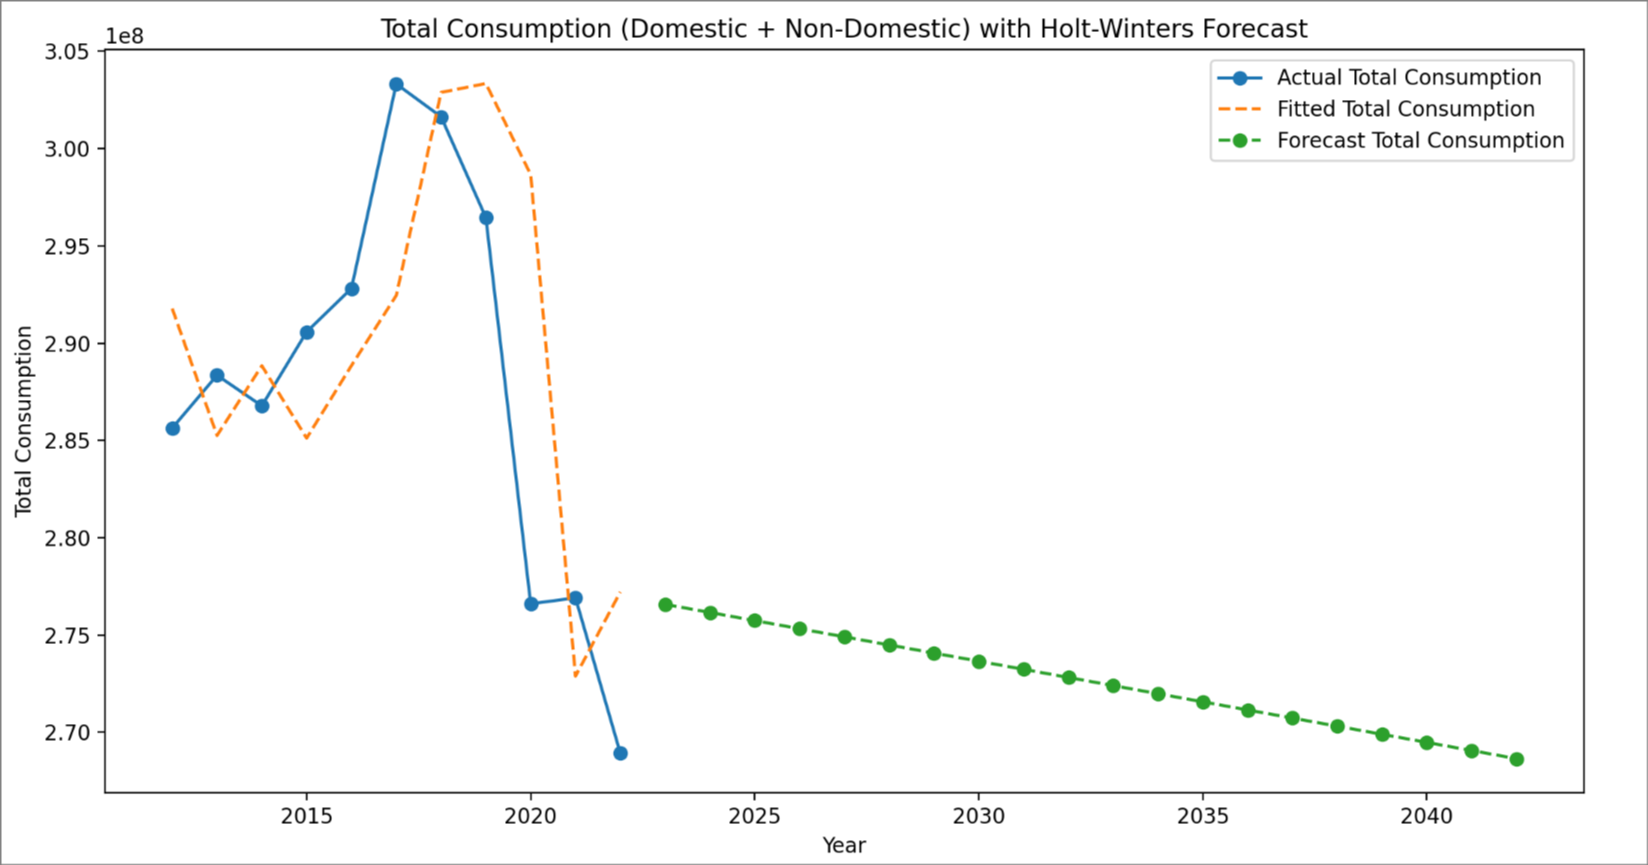
\includegraphics[scale=0.25]{Images/Q2.png}
  \caption{Plot of the actual total energy consumption with our modelled total energy consumption and forecast total energy
  consumption in summer months.}
\end{figure}
\end{center}

\subsection{Discussion of results}

From analysing the plots of the graphs in figure 2, we can see that our fitted model is rather accurately predicting the
total energy consumption in summer months from 2012 to 2022, with a small amount of lag. After 2022 our forecast prediction
continues the decreasing trend demonstrated in the last few years, without any of the fluctuations shown in the data set.

This model accurately captured the general direction of the data set. However since the forecasted data doesn't have the same
fluctuations as the data set given, it doesn't seem unreasonable to conclude that the accuracy and certainty of our
predictions could be considered dubious.

\section{Q3: Beat the Heat}
\subsection{Problem statement}

In Q3 we interpret the problem statement like so:

Develop a system to determine a vulnerability score which can be assigned to a  variety of neighborhoods. Depending on the score, the neighborhoods will be allocated a sufficient amount of resources to reduce the effects of a heat wave or power grid failure. Include an approach of how Birmingham can use these scores in their process of managing heat waves.

\subsection{Assumptions}
\textbf{\sffamily We assume that the wind speed is constant}

\textit{Justification:} Since the rate at which a person cools is directly proportional to the wind speed, i.e. the faster the wind speed the faster a person will be able to cool. Thus, in order to eradicate this parameter and simplify the problem this will be assumed to be constant.

\noindent
\textbf{\sffamily We assume that the people in Birmingham are static, that is they have negligable movement throughout the entire 24 hours}

\textit{Justification:} A person's body temperature will heavily affect the heat index which will be calculated so by minimizing ones movement the value of the heat index will be of higher accuracy, in other words it will provide a better representation of how hot a particular person feels throughout the 24 hour heat wave in Birmingham.

\noindent
\textbf{\sffamily We assume that the power outages will occur during the summer months}

\textit{Justification:} By applying this assumption within our model we will be able to effectively use the Heat Index as a vulnerability parameter.

\subsection{Analysing the problem}

By studying the following article, \textit{'Predicting Indoor Heat Exposure Risk during Extreme Heat Events'} \cite{indoorheat}, it was clear that we would use the Heat Index as a suitable vulnerability score. The Heat Index effectively quantifies how hot a human body will feel at a particular temperature and humidity \cite{indoorheat}. Thus, it is an important factor in terms of determining what areas will need additional support and resources during a heat wave. It is also an effective parameter to minimize effects during power outages. For example, by observing a variety of Heat Index values at particular points in time during a day we will be able to determine what parts of the city are being affected by hot temperature the most and allocate a suitable amount of power to this part of the city rather than other parts during these times and at other times other parts of the city may be affected more - so suitable resources can be allocated to these parts instead.

In order to achieve this we will make use of the Heat Index Equation where the key assumptions for this equation have been explained above. The equation is as follows \cite{HIformula}:

\[
\begin{aligned}
\gamma &= -42.379 + 2.04901523 \ T + 10.14333127 \ \text{RH} \\
&\quad -0.22475541 \ T \ \text{RH} - 0.00683783  \ T^2 \\
&\quad - 0.05481717 \ \text{RH}^2 + 0.00122874\ T^2 \ \text{RH} \\
&\quad + 0.00085282 \ T \ \text{RH}^2 -0.00000199 \ T^2 \text{RH}^2
\end{aligned}
\]

However, we need to calculate the Relative Humidity for each value of Humidity given, this is calculated by the following \cite{relativeHumidity}:

\[
\epsilon = 100 \times \left[ \frac{\exp\left(\frac{17.625D_p}{243.04+D_p}\right)}{\exp\left(\frac{17.625T}{243.64+T}\right)} \right]
\]

\subsection{Variables and parameters}

\begin{longtblr}[
  caption={Variables and parameters.}
]{
  colspec={llX},
  row{1}={lightgray}
}
Name & Notation & Description \\

Relative Humidity & $\epsilon$ & Measure of the water content in the air compared to the maximum water content that the air can hold at a particular temperature. \\

Temperature & $T$ & Temperature of the air in degrees celcius. \\

Heat index & $\gamma$ & A measure of how hot the air temperature feels at a particular temperature and humidity. \\

Dew point temperature & $\rho$ & The temperature in degrees celcius at which air holds the maximum amount of water vapour \\

\end{longtblr}


\subsection{Developing the model}
Define $\gamma$($\epsilon$, \text{T}) to be the function that calculates the heat index at any temperature, T, and relative humidity, $\epsilon$. Let $\epsilon$($\rho$, T) to be the function that calculates the relative humidity at a particular value of $\rho$ and T. Again, we will make use of the data set given in the M3 \cite{m3}, which gives the values for $\rho$ and T over the 24 hour time period of the heat wave.

Here is a snippet of the algorithm: \textit{Full code can be viewed in appendix}

\begin{minted}[bgcolor=lightgray, linenos, breaklines]{python}
import math
import matplotlib.pyplot as plt

# Calculating Relative Humidity
def CalcHumidity(airTemp, dewPointTemp):
    top = math.exp( (17.625 * dewPointTemp) / (243.04 + dewPointTemp) )
    bottom = math.exp( (17.625 * airTemp) / (243.04 + airTemp) )
    newHumidity = (top / bottom) * 100
    return newHumidity

# Calculating corresponding Heat Index
def CalcHeatIndex(airTemp, newHumidity):
    calculatedIndex = -42.379 + 2.04901523 * airTemp + 10.14333127 * newHumidity - 0.22475541 * airTemp * newHumidity - 0.00683783 * (airTemp**2) - 0.05481717 * (newHumidity**2) + 0.00122874*(airTemp**2) * newHumidity + 0.00085282 * airTemp * (newHumidity**2) - 0.00000199 * (airTemp **2) * (newHumidity**2)
    return calculatedIndex

...
plt.show()
\end{minted}

Here is the output of the code:

\begin{center}
\begin{figure}[H]
  \centering
  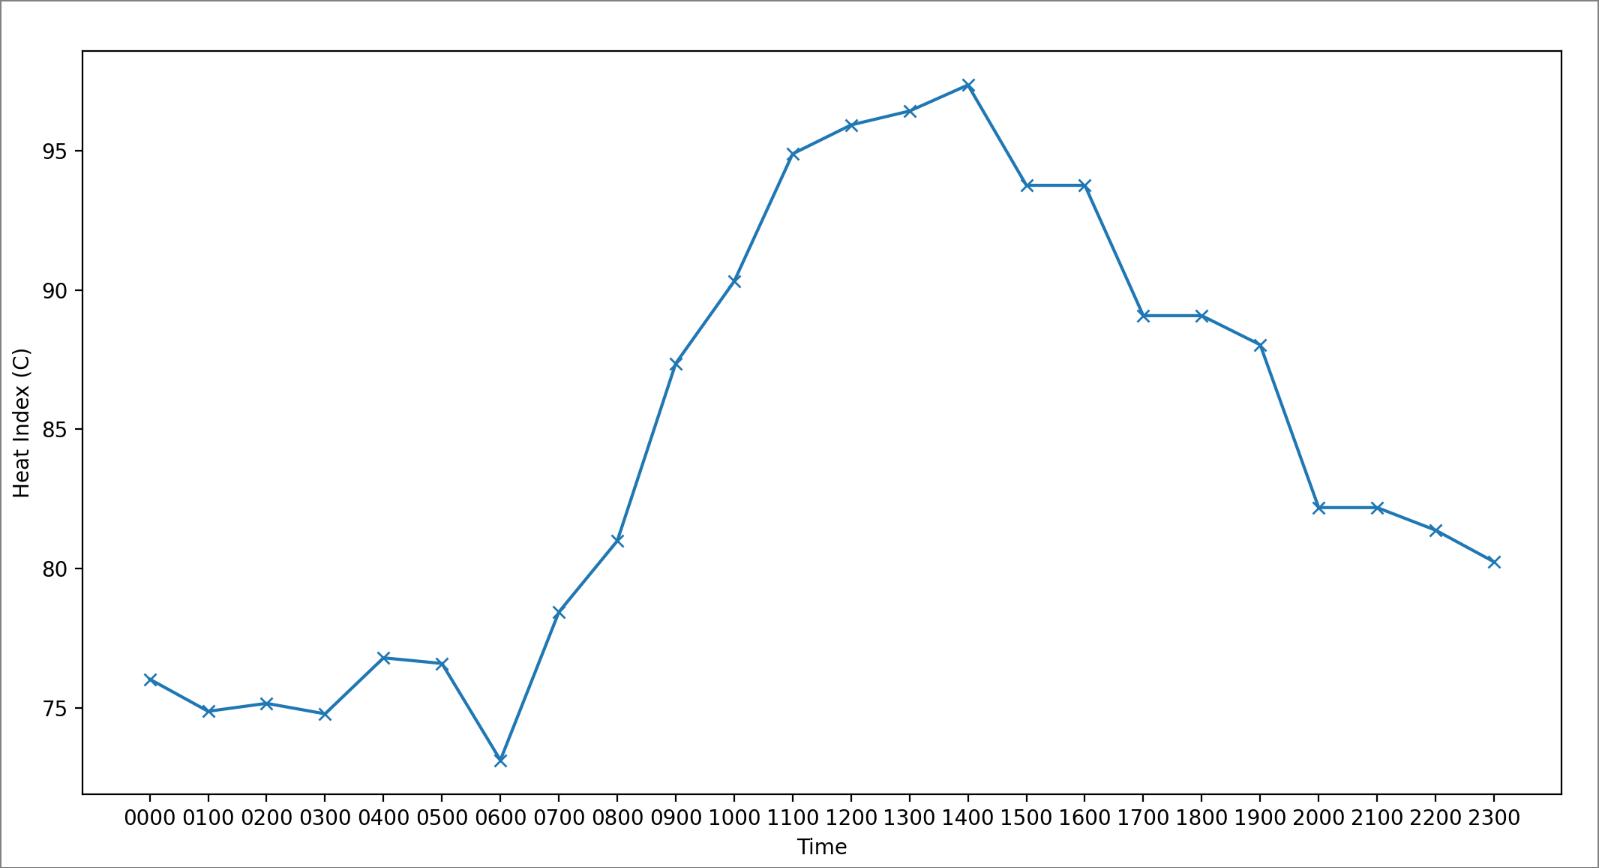
\includegraphics[scale=0.25]{Images/Q3.png}
  \caption{Plot of the heat index against time.}
\end{figure}
\end{center}


\section{Appendix}

\subsection{Q1}

\inputminted[bgcolor=lightgray, breaklines, linenos]{python}{./Code/Q1.py}

\subsection{Q2}

\inputminted[bgcolor=lightgray, breaklines, linenos]{python}{./Code/Q2.py}

\subsection{Q3}

\inputminted[bgcolor=lightgray, breaklines, linenos]{python}{./Code/Q2.py}

\newpage
\printbibliography

\end{document}
